\chapter{Study}

This chapter gives an overview of the literature survey and investigation done for this project. We also discuss the reasoning behind some of the important design decisions.
%The major activity in this chapter is literature survey, investigation
%and arriving at the targetted scope and specifications. Here the 'what',
%'why' and 'how' of the product and product sub-parts are studied.
%One looks for similars in already existing products and makes comparisons.
%One identifies potential decisions that need to be taken with respect
%to the product evolution and performs a comparative statement of possible
%options that will affect design decisions. 

%NOTE: While discussing the various options and the comparisions, you
%need to cite appropriate references at appropriate places in the text.
%A typical \emph{citation} \cite{paper1,paper2,paper3,paper4,paper5,paper6} is
%referred as shown here. The cited references will automatically be
%reflected in the bibliography section in the order of occurence of
%citation in the manuscript. A sample \emph{report.bib} file is included
%in this template. Kindly go through it and make your bibliography
%file accordingly. A free software like \emph{JABREF} (a java application)
%or \emph{ZOTERO} (a firefox addon) can be used to create your bibliography
%file.


\section{Functional concept}
The \emph{PanicButton device} has to perform tasks like take user's input from the panic button, acquire audio data needed for audio-based trigger, communicate with the back-end server and user's smartphone, detect any tampering and run audio processing algorithms. Figure~\ref{fig:functionalDesc} and  figure~\ref{fig:functionalDescbus} shows the top level functional diagram of the \emph{PanicButton device} when installed in cabs/autos and bus respectively.

\emph{PanicButton device} is equipped with a panic button to take user inputs, bluetooth low energy (BLE) for communicating with the user's smartphone, global system for mobile communication (GSM) to communicate with back-end server, global positioning system (GPS) to locate the vehicle in case of emergency, microphone to record audio and speaker to play audio.

Users can validate \emph{PanicButton device} using their smartphone through a dedicated android application. Communication between the user's smartphone and the \emph{PanicButton device} is handled by the respective BLE module. After performing validation, user is notified with the status of microphone, emergency button, firmware and enclosure of the system.

%\begin{figure}[H]
%\centering
%\def\svgwidth{\textwidth}
%\input{functionalDescription.pdf_tex}
%\caption{Functional description of connected panic button with audio-based trigger}
%\label{fig:functionalDesc}
%\end{figure}

%\begin{figure}[H]
%\centering
%\def\svgwidth{\textwidth}
%\input{bus.pdf_tex}
%\caption{Functional description of connected panic button with audio-based trigger inside a bus}
%\label{fig:functionalDescbus}
%\end{figure}
\begin{figure}[H]
\centering
\def\svgwidth{\textwidth}
\includegraphics[width=0.9\textwidth]{functionalDescription}
\caption{Functional description of the \emph{PanicButton device} with audio-based trigger in auto/cab}
\label{fig:functionalDesc}
\end{figure}

\begin{figure}[H]
\centering
\def\svgwidth{\textwidth}
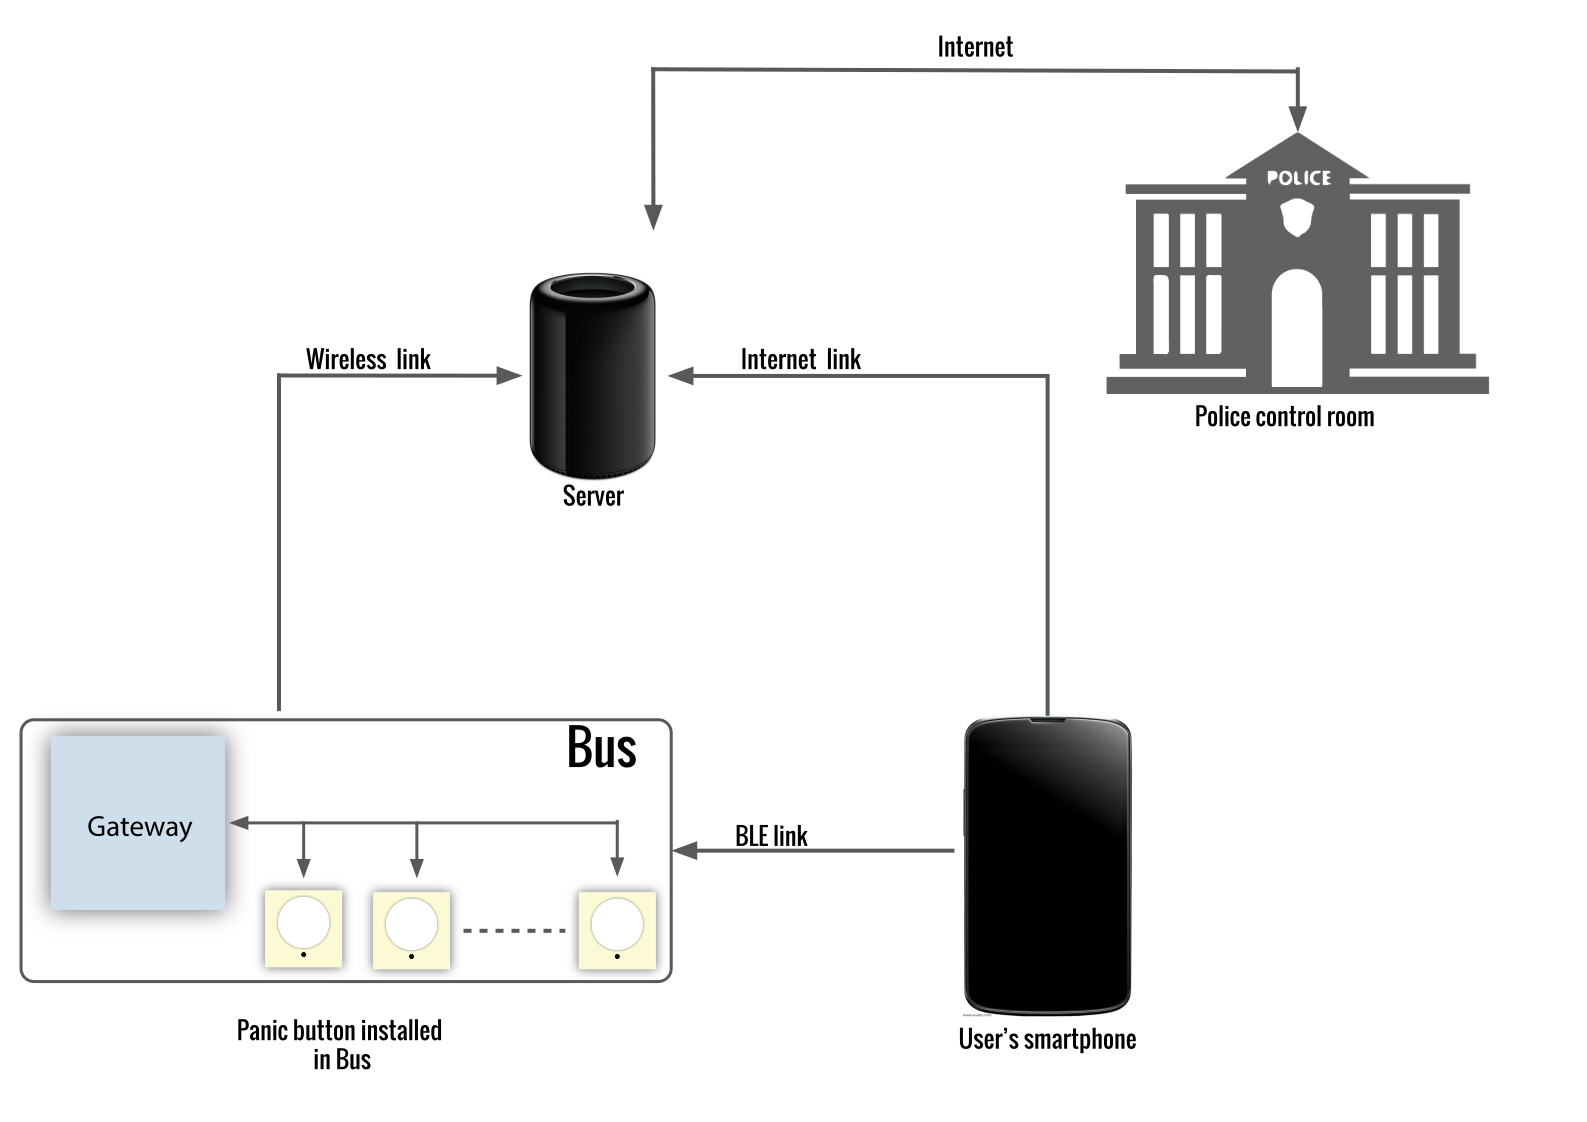
\includegraphics[width=0.9\textwidth]{bus}
\caption{Functional description of the \emph{PanicButton device} with audio-based trigger in bus}
  \label{fig:functionalDescbus}
\end{figure}

Emergency is asserted, if either the panic button is pressed or scream is detected by audio-based trigger. In case of emergency, compressed stream of audio along with vehicle's location is sent to the server, for later examination.


%This should include 
%\begin{itemize}
%\item a discussion on the product with the aid of block diagrams and figures
%\item an exhaustive list of stimuli to product
%\item classification of the stimuli as input/output, power signal/information
%signal, electric/mechanical etc.
%\item First level quantification of the stimuli like, voltage levels, type
%of signals (dc, ac, pulsed), rise time, current levels, etc.
%\end{itemize}

\section{Module study}
This section dwells in literature survey and design decision done for the individual modules.

\subsection{Protocols for communication}
We studied the protocols that can be used between the links present in the system. There are four different links in the system.
\begin{itemize}
\item link between the \emph{PanicButton device} and the back-end server,
\item link between the smartphone and the back-end server,
\item link between the smartphone and the \emph{PanicButton device},
\item link between the back-end server and the PCRs.
\end{itemize}
The following subsections will go into the details of each of them.
\subsubsection{Protocol for messaging between the \emph{PanicButton device}, the back-end server and PCRs}
The message link between panic button and back-end server must be a low latency link. In order to achieve that we looked at different protocols with their merits and demerits. The following protocols can be used for this link.
\begin{itemize}
\item Hypertext Transfer Protocol 1.1 (HTTP)
\item Message Queue Telemetry Transport (MQTT)
\item Constrained Application Protocol (CoAP)
\end{itemize} 
HTTP is one of most widely used protocol for data transfer. It is the foundation of data communication for the World Wide Web (WWW). HTTP is a text based application layer protocol, which uses Representation State Transfer (REST) with four methods \emph{GET}, \emph{PUT}, \emph{POST} and \emph{DELETE}.\\
MQTT is one of the emerging protocol in the Internet of Things(IoT) domain. MQTT uses Transmission Control Protocol(TCP) as transport layer. It uses publish subscribe pattern with only two methods \emph{SUBSCRIBE} and \emph{PUBLISH}. MQTT is a protocol with very small header overhead.\\
CoAP is another IoT protocol designed specifically to be used in the lightweight environments.  CoAP is designed to easily translate to HTTP for simplified intergration with the web. CoAP runs over User Datagram Protocol (UDP) transport layer.\\
Table~\ref{tab:mess_procotols} compares different protocols.
\begin{table}[H]
\begin{center}
\begin{tabular}{ |c|c|c|c|c| } 
 \hline
 \textbf{Protocol} & \textbf{REST/PubSub} & \textbf{Transport layer protocol} &\textbf{header} & \textbf{Min-header (bytes)} \\
 \hline 
 \hline
 HTTP & REST & TCP & Text & 18 \\
 \hline
 MQTT & PubSub & TCP & Binary & 2 \\ 
 \hline
 CoAP & REST & UDP & Text & 4  \\ 
 \hline
\end{tabular}
\end{center}
\caption{Camparision of HTTP, MQTT and CoAP} \label{tab:mess_procotols}
\end{table}
The architecture of the our system can benefit from publish subscribe model for transparent transfer of messages between the \emph{PanicButton device} and PCR, where back-end server will act as a message broker. The back-end server can relay messages transparently to different PCRs at different locations. MQTT uses binary header with smallest packet size of just 2 bytes, which helps in reducing the bandwidth requirement for the communication. 
\subsubsection{Protocol for audio streaming}
The audio stream link between the \emph{PanicButton device} and back-end server requires high throughput, low latency, guaranteed delivery link. The protocols under consideration are
\begin{itemize}
\item HTTP1.1 over TCP
\item Raw over TCP
\item Raw over UDP
\end{itemize}
We decided to use raw over TCP because it fulfills the requirements for this link. HTTP 1.1 also provides the same benefits as raw over TCP, but adds large header overhead which is not desired. The extra information regarding the stream can be embedded in the compressed audio stream explained in the next section.
\subsection{Compression algorithm}
\label{sec:compression}
The use of wireless link from the \emph{PanicButton device} to the back-end server restricts the bandwidth which is available for audio transmission. The compression of audio stream is essential for reliable transfer of audio from panic button to back-end server under congestion.\\

\begin{table}[H]
\begin{center}
\begin{tabular}{ |c|c|c|c| } 
 \hline
 \textbf{Format} & \textbf{Lossless} & \textbf{Compression factor} &\textbf{Open-source/royalty-free} \\
 \hline 
 \hline
 Raw & Yes &  1:1 & Yes\\
  \hline
 Wav & Yes &  1:1 & Yes\\
 \hline
 Mp3 & No &  5:1 & No\\
 \hline
 Vorbis Ogg & No &  10:1 & Yes\\
 \hline
\end{tabular}
\end{center}
\caption{Expermental comparision of different audio formats at 44100 sample rate and 16-bit per sample} \label{tab:audio_formats}
\end{table}
Different audio formats are experimentally compared in table~\ref{tab:audio_formats}. Vorbis is open-source, royalty free audio compression and streaming format. Vorbis ogg's performance is better compared to mp3 in terms of compression ratio. We decided to use Vorbis Ogg audio format for streaming audio from the \emph{PanicButton device} to the back-end server.
\subsection{Encryption algorithm}
%\subsubsection{Encryption between panic button and back-end server}
Encryption is used to avoid man-in-the-middle attacks between the  \emph{PanicButton device} and the back-end server. Two of the most popular encryption algorithms are Advanced Encryption Standard (AES) and RSA algorithm. RSA algorithm uses asymmetric key configuration, while AES algorithm uses symmetric key configuration. The advantage of using RSA algorithm over AES is that, even if public key(key stored in panic button) is compromised, the communication is not compromised.
We decided to use RSA over AES due to this advantage.
%\subsubsection{Encryption between enclosure tamper detection module and core-module}

%\subsection{System validation module}
%One of the most essential part of the system is to have a self check mechanism to ensure the full functioning of the system. In case an anomaly is found in the system, it should notify the user as well as the back-end server.\\
%The panic button is installed in the public transport which makes it very vulnerable to tampering. There are number of ways in which it can be tampered. Few of them are
%\begin{itemize}
%\item Removing the power source from the panic button.
%\item Tampering with the physical button.
%\item Tampering with the microphone.
%\item Tampering with the enclosure.
%\item Physically change in the circuit.
%\item Change in firmware of the micro-controllers.
%\item Replacing the entire system with a dummy one.
%\item Swapping two system with each other.
%\end{itemize}
%The system must be able to detect any kind of tampering, in order %to keep the trust intact with the users.\\
%We propose few tamper detection mechanisms, which can warn the %user while boarding.
%\subsubsection{Enclosure tamper detection}
%In order to detect tampering with the system, unauthorized access to internal circuitry and components must be detected. To handle this undesirable event we looked at following methods.
%\begin{itemize}
%\item An ultra low power push button based detection system, %which will change the state of button if somebody tries to open %the enclosure.
%\item An ultra low power wire based detection system, which will %break if somebody tries to open the enclosure.
%\end{itemize}
%In push button based detection system, push button will be %installed inside the enclosure, which will be enabled as soon as %enclosure opens.\\
%In wire based detection system, wire runs around the periphery of %the enclosure, which will permanently break as soon as enclosure %opens.\\
%Tamper detection module must be always-on, independent of the %power source availability. It must have battery life of atleast %few years for tamper detection to work reliably.\\
%The tamper detection module must retain state independent of %change the firmware or change of the component. In order to %achieve that the core-module must detect that change. We propose %to store secret private key in tamper detection module and core-%module. The communication between the core-module is encrypted so %that third party can't watch the exchange of messages. In case of %tamper, tamper detection module permanently deletes his copy of %private key.\\
%Advanced Encryption Standard (AES) algorithm is not appropriate %for ultra low power microcontroller. A tiny footprint encryption %algorithm is required to encrypt the messages transfered between %core-module and tamper detection module.\\
%Tiny Encryption Algorithm (TEA) is a encryption algorithm %suitable for ultra low power microcontroller. Instead to relying %on complicated operation, it uses large number of iterations of %simple operations\cite{tea_paper}. We used Modified Tiny %Encryption Algorithm (MTEA), which is based on TEA with 16-bit %operations instead of 32-bit operations.
  



\subsection{Audio-based trigger module}
This audio-based trigger comes under \emph{sound event detection} domain of relatively broad research area of audio/sound analysis. Sound event detection is relatively new area compared to speech analysis, so most of the literature in the field of acoustic analysis is highly clustered around speech analysis. In section~\ref{sssec:featforscream}, we take a look at literature survey and experiments done to come up with required feature for scream detection; in section~\ref{sssec:algoforscream}, we take a look at literature survey done for algorithm to be used for scream detection.

\subsubsection{Feature for scream detection}
\label{sssec:featforscream}
Features extracted from acoustic signals are vectors that can faithfully represent them. In order to develop the best possible classification algorithm for reliable detection and classification of sound events, it is very important to select the feature set carefully. Although a large feature set has its benefits of generating accurate results, using a small feature set can reduce latency and make the design simpler.

Over the last few years, several audio feature extraction techniques have been introduced. They make use of one of the following two signal representation domains: temporal
and spectral. Temporal domain features such as signal energy, pitch, zero-crossing \cite{paper4} rate and entropy modulation \cite{paper5} have been used for speech classification but are not enough to represent the non-stationary characteristics of sound events. Spectral features such as percentage of low energy frames, 4-Hz modulation energy, spectral roll-off point, mean frequency, spectral centroid, mel-frequency cepstral coefficients and frequency slopes are useful in audio classification, but they do not provide any information about the temporal evolution of the extracted features over the frame.

Initially researchers used popular mel-frequency cepstral coefficients (MFCC) as features for sound event detection. MFCC are short-term spectral based features. These features are extracted through a series of digital signal processing steps like windowing, Discrete Fourier Transform(DFT), logarithm and Discrete Cosine Transform (DCT). MFCC are still used for non-verbal sound recognition \cite{paper6}. A paper\cite{paper7} proposed a sound event classifier which use MFCC feature set; they achieved 74\% accuracy. Another paper \cite{paper8} successfully classified acoustic environmental sounds like office, soccer match, beach, laundrette, street noise, rail station, car, bar and bus using a Hidden Markov Model(HMM) based classifier which used MFCC as feature vectors.

%TODO ref for LPC
Linear predictive coefficients (LPC) is another well known feature set used for sound
classification of car noise, factory noise, street noise, babble and bus noise. A Quadratic
Gaussian classifier using LPC feature set gives accuracy of 90\% for car/factory noise
and 60-80\% for the rest.

Time-Frequency Matrix(TFM) feature set tends to capture non-stationary and discontinuous properties of sound events. This matrix is obtained using matching-pursuit time-frequency distribution (MP-TFD) technique, followed by non-negative matrix decomposition to decompose the TFM into its significant components \cite{paper9}.

After looking at individual feature sets, researchers started fusion of various feature sets. \cite{paper6} used MFCC along with Pitch range based features, \cite{paper10} used MFCC along with spectral features like centroid, flux, flatness, roll-off, harmonic-to-noise ratio and pitch. TFM when combined with a few spectral and MFCC features, gives 10\% accuracy-rate improvement compared to only MFCC features based classifiers \cite{paper9}.

One paper \cite{paper11} went in completely different direction to tackle the issue of sound event classification, they argued that sound events produced a unique texture, which can be visualized using a spectrogram image and could be analyzed for automatic sound event detection. Another paper \cite{paper12} used pseudo-coloration to enhance the perception. Spectrogram is first normalized into grey-scale with a fixed range, then dynamic range is quantized in to regions, each of which is then mapped to form a monochrome image. Finally monochrome images are partitioned in to blocks and distribution statistics in each block are extracted to form the feature set. Robustness of spectrogram based methods comes from the fact that noise
is normally more diffused than the signal and therefore the effect of noise is limited to a
particular quantization region, leaving other regions less effected.

Feature used in detection/classification systems impacts their response time and power
consumption. A non-realtime application can make use of large and time consuming feature sets to get highly accurate results, while a realtime application can only use feature
set that fit into its time budget. Power consumption is important aspect in battery powered devices; Feature set that can give acceptable accuracy at lesser computation results in system that lasts longer on a single charge.

We decided to use MFCC along with spectral features like centroid, flux, flatness, roll-off, harmonics-to-noise ratio and pitch due to its promising performance \cite{paper10}. We conducted an experiment to find out the execution time of this feature set. The task of detecting scream is to be performed in real-time. In our project we decided to analyze live audio stream every 1 second, which gives us 2 second to analyze and give results for audio received in previous second, this decision was based on the analysis done by \cite{paper10}, which showed average scream duration to be around 2 second. We tried MFCC plus few spectral features as feature vector and computed feature extraction time for an audio clip of 2 second, Table~\ref{tab:scr2} summarizes scream detection time on two hardwares.

\begin{table}[H]
\begin{center}
\begin{tabular}{ |c|c| } 
 \hline
 \textbf{Platform} & \textbf{Feature extraction time (in s)} \\
 \hline 
 \hline
 Raspberry pi 3 & 13 \\
 \hline
 Intel quad core i5-4440 @ 3.10GHz (16 GB) & 1.5 to 2 \\ 
 \hline
\end{tabular}
\end{center}
\caption{Feature extraction time using MFCC and spectral feature as feature vector} \label{tab:scr2}
\end{table}

With MFCC and spectral features as feature set, we had latency of 13 sec which is beyond the 2 sec limit. We had to shed computationally expensive part of this composite dataset to squeeze into the budget of 2 sec, we decided to use only MFCC as feature vector and Table~\ref{tab:scr1} summarizes the execution time of this dataset.

\begin{table}[H]
\begin{center}
\begin{tabular}{ |c|c| } 
 \hline
 \textbf{Platform} & \textbf{Feature extraction time (in s)} \\
 \hline 
 \hline
 Raspberry pi 3 & 1.480 \\
 \hline
 Intel quad core i5-4440 @ 3.10GHz (16 GB) & 1.020 to 1.050 \\ 
 \hline
\end{tabular}
\end{center}
\caption{Feature extraction time using MFCC as feature vector} \label{tab:scr1}
\end{table}

With MFCC as feature vector we have latency of 1.480 sec, which is less than our time limit of 2 sec. We decided to go with MFCC as the feature vector for scream detection.

\subsubsection{Classification algorithm for scream detection}
\label{sssec:algoforscream} 

These algorithms take features as input and output probabilities of all classification class for the given input. The class with highest probability for a given input is said to be the class of the input.

Initially researchers used classifiers like a quadratic Gaussian classifier, a least-square
linear classifier, a neighbor classifier and a decision tree classifier \cite{paper6}. These classifiers could preform well for particular sound events but couldn't generalize well to non-verbal sound events.

Lately researches have started using machine learning for the purpose of sound event classification. Algorithms like Artificial Neural Network (ANN) \cite{paper6} and Support Vector Machine(SVM) \cite{paper10} are being used widely. These algorithms fall under the category of supervised machine learning. These algorithms outperform nearly all other classifiers used in past due to their capability to model complex systems.

ANNs are mathematical models that emulates biology of a human brain. ANNs are parallel computing mechanisms that contains neurons laid out as a layers, interconnects and learning rules. SVMs are another set of mathematical models used for classification. SVMs constructs a hyperplane or set of hyperplanes in a high dimensional space, which is used for classification. ANN algorithms require more data to train the classifier as compared to SVMs. In case of SVMs, we need to set a limited number of parameters and choose among possible kernel. We decided to use SVM algorithm due to available limited dataset and easy convergence in training. 

%For each of the modules, include
%\begin{itemize}
%\item an exhaustive list of stimuli to the module
%\item classification of the stimuli as input/output, power signal/information
%signal, electric/mechanical etc.
%\item First level quantification of the stimuli like, voltage levels, type
%of signals (dc, ac, pulsed), rise time, current levels, etc.
%\end{itemize}

%\subsection{Sub-modules}

%If necessary, partition the various modules into sub-modules and %so
%on till the component level. 

%\emph{NOTE}: At every module, sub-module or component level (electric
%hardware or algorithms or industrial design), if there are multiple
%options available, then perform a comparative study of the most significant
%features among the options to evaluate the merits and demerits of
%the various options. Based on the merits and demerits of the various
%options, give your recommendations for design.


\section{Industrial design}
Being a product for public safety service, it should blend with the vehicular environment yet remain accessible. The panic button mounted on the \emph{PanicButton device} has to be easily accessible 24x7. A button with area equal to the average area of adult hand and back-light will fulfill these requirements. Front panel of the \emph{PanicButton device} mounts three essential part namely panic button with status back-light, speaker and microphone. Front panel also acts as lid for the \emph{PanicButton device}. Secondary battery and electronics used in this project resides at the base of enclosure. Figure~\ref{fig:baselayout} shows a pictorial representation of the assembly.

\begin{figure}[H]
\centering
\includegraphics[width=\textwidth]{base_layout}
\caption{Layout of battery and electronics at the base of the \emph{PanicButton device}}
\label{fig:baselayout}
\end{figure}  

Details of this enclosure will be covered in Industrial design section of chapter 3.


%The industrial design/product design aspects should consider the following,
%\begin{itemize}
%\item Design mix - functional, ergonomics and aesthetics aspects of the
%product should be discussed giving consideration to appropriateness
%to a given application.
%\item Layout - the layout of the modules and the sub-modules within an enclosure
%or system should be discussed as determined by the following considerations, 

%\begin{itemize}
%\item user, form, ergonomics, aesthetics, interconnections, display, etc.
%\item realisation issues of a particular layout
%\item functional aspects like EMI, thermal, wiring etc.
%\end{itemize}
%\item Product structure - provide a discussion on the product generic structure,
%whether it should be

%\begin{itemize}
%\item rack and frame mounted 
%\item modular cabinet
%\item non-modular
%\item custom 
%\end{itemize}
%\item Materials - provide a discussion on the choice of materials for the
%product
%\item Manufacturing processes
%\item Cost of the product
%\end{itemize}

%\section{Target scope}

%The following questions need to be addressed:
%\begin{itemize}
%\item What is the targetted scope of the product?
%\item What is the set of target specifications to design the product?\end{itemize}

